\documentclass{article}
\usepackage{import}
\subimport{../}{preamble}
\begin{document}

%\fullcite{bharadwaj2009}

\section{Plasmons in Tips}
\label{sec:tip_literature}

Significant efforts have been made to advance surface characterisation on the nm-scale by developing new optical tools and integrating optics into existing nanoscale topological measurements. Metallic tips were therefore investigated due to the widespread use of \glspl{spm}, such as \gls{afm}, and \gls{stm}. The similarity in size between metallic nanostructures and the small apex of tips initially suggested that visible plasmons would be expected, enabling resonant near-field enhancement.
% Application of tips to TERS and SNOM - keep this short, the thesis is not about Raman but this is a motivation
Prior to any spectral characterisation studies to understand the near-field response, tips were applied in combined SPM-optical microscopes to achieve sub-wavelength localisation and enhancement of optical signals. As the next logical step from \gls{sers} and \gls{snom}, the sharp apex of tips were exploited to develop the spin-off techniques of \gls{ters} \cite{stockle2000, anderson2000, hayazawa2000, pettinger2000} and apertureless/scattering scanning near-field optical microscopy (a-SNOM/s-SNOM) \cite{zenhausern1994, zenhausern1995, bachelot1995, knoll1997, knoll1998, keilmann1999}. These are also known collectively as \gls{tenom}.%
\footnote{These are also sometimes known as field-enhancing near-field optical microscopy (FENOM) since apertured techniques do not necessarily exploit plasmonic enhancement as much.}

% TERS
The concept for TENOM was first proposed in 1985 \cite{wessel1985} but it was not until 2000 that the first reported uses of tips for enhancing Raman spectroscopy emerged \cite{stockle2000, anderson2000, hayazawa2000, pettinger2000}. Two of the initial measurements suggested the overall Raman enhancement has a \emph{lower limit} of $10^4$ \cite{stockle2000, anderson2000}, hence a field enhancement of order 10, whereas a third demonstrated that a single tip apex has the equivalent enhancement of the sum of many SERS hotspots on a Ag island film \cite{hayazawa2000}. All measurements were carried out in inverted microscopes with either an AFM \cite{stockle2000, anderson2000, hayazawa2000} or STM \cite{pettinger2000} {\color{red}setup} mounted on top.
Near-field evanescent wave coupling using $\mathit{NA}>1$ resulted in a field enhancement of 80 \cite{hayazawa2000}. Since then field enhancements of up to \num{e7}--\num{e9} have been measured \cite{}.

\begin{figure}[h]
%\centering
\flushleft
\fontsize{10pt}{1em}\selectfont
\begin{subfigure}[t]{0.47\textwidth}
	%\centering
	\subimport{./figures/}{tenom_basic}
\end{subfigure}
~
\begin{subfigure}[t]{0.49\textwidth}
	%\centering
	\subimport{./figures/}{tenom_surface}
\end{subfigure}
\caption[Concepts of TENOM]{\textbf{Concepts of TENOM.}
Tips can perturb evanescent surface waves and scatter them into the far-field ($1\rightarrow3$) \cite{neacsu2005, mehtani2006}.
Photons illuminating a tip-sample junction can induce a hot-spot, which scatters light into the far-field ($2\rightarrow3$).
SPPs coupled onto a planar metal surface (via a tip) can radiatively decay into $\mathit{NA}>1$ ($1\rightarrow4$) \cite{wang2011}.
{\color{red}Mechanism ($2\rightarrow4$) has not been attempted.}}
\label{fig:tenom_concept}
\end{figure}

%\begin{figure}[h]
%\centering
%\begin{subfigure}[t]{0.45\textwidth}
%	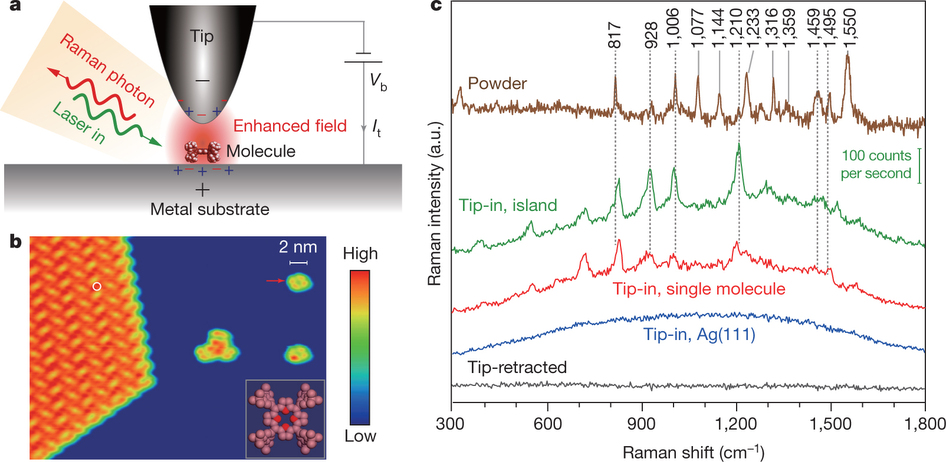
\includegraphics[width=\textwidth, clip=true, trim=0 240 550 15]{figures/literature/nature12151-f1_2}
%	\caption{An example of a side-illumination experimental TERS geometry used for chemical mapping of single molecules \cite{zhang2013}.}
%\end{subfigure}
%~
%\begin{subfigure}[t]{0.45\textwidth}
%	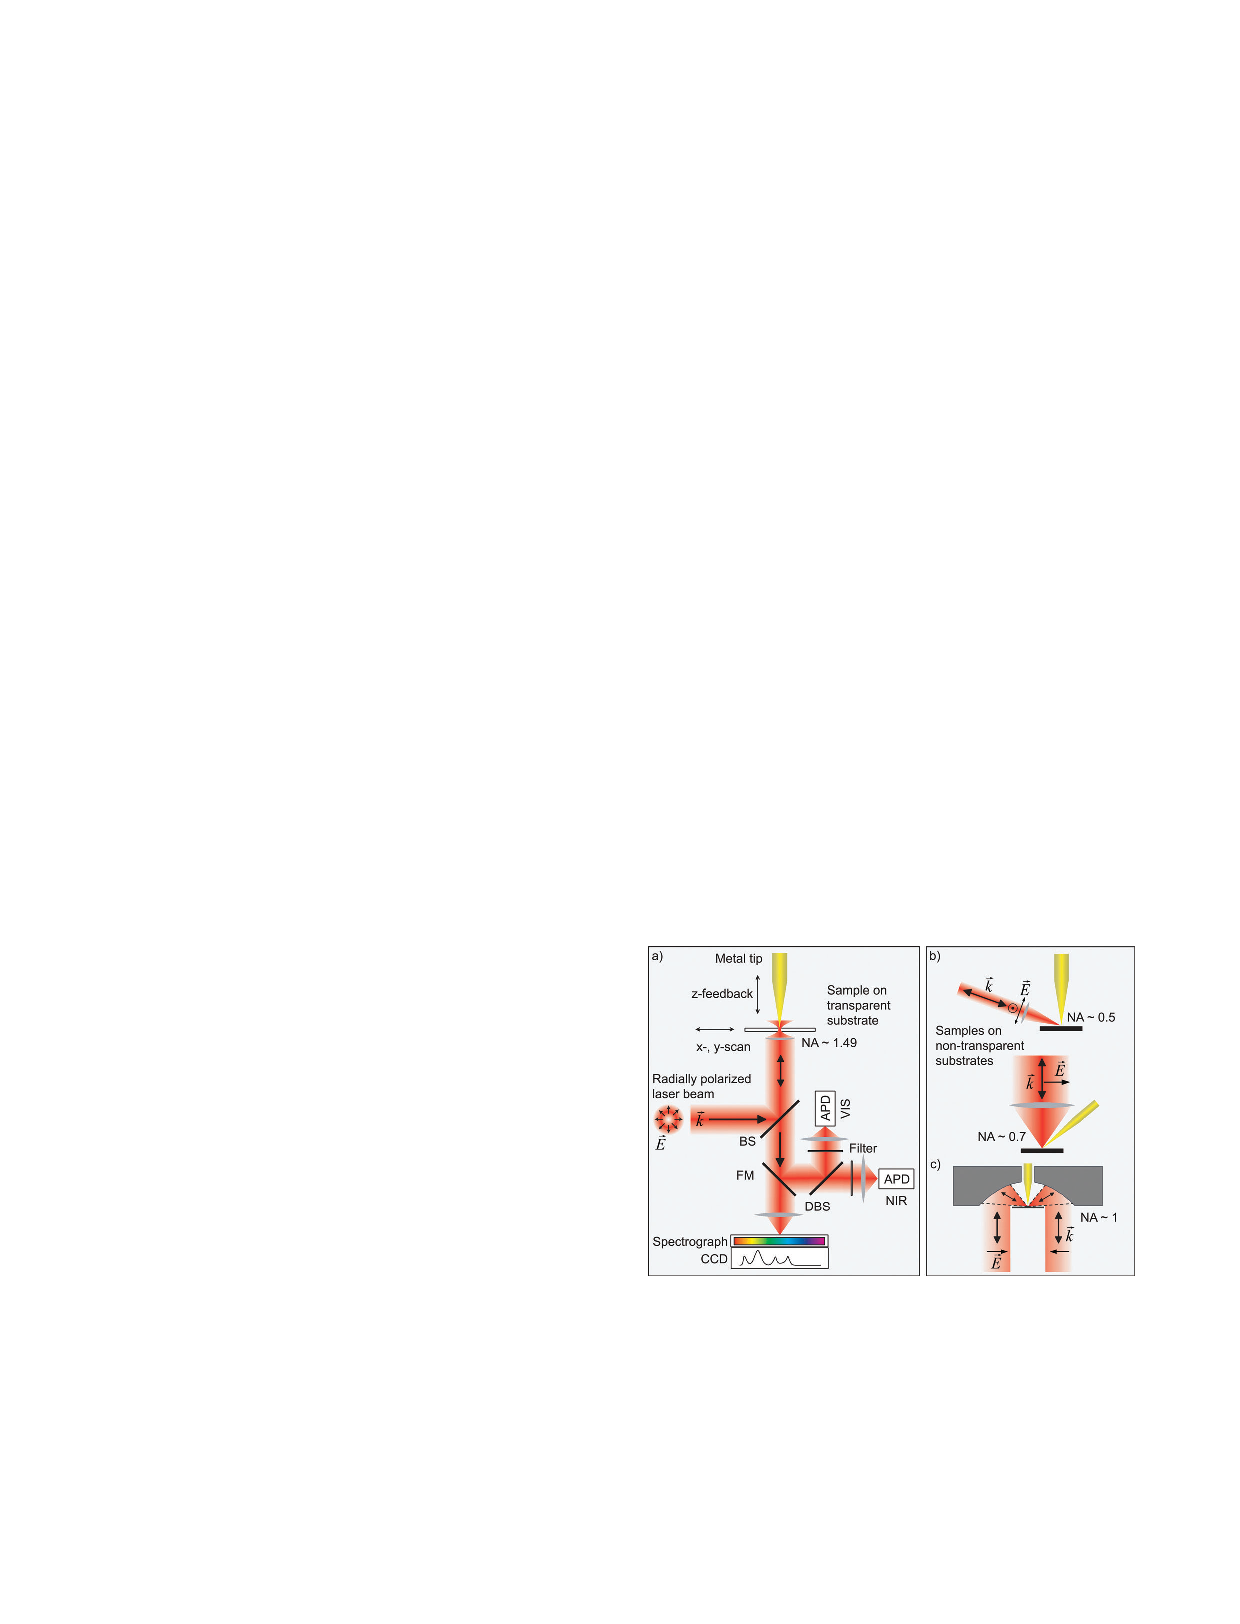
\includegraphics[width=\textwidth]{figures/literature/mauser2014a}
%	\caption[]{Typical optical geometries found in TENOM experiments \cite{mauser2014}. The most prominent system is the bottom-illumination/back-illumination configuration utilising high-NA objectives. The other main geometry is the side-illumination configuration.}
%	\label{fig:ters_geometries}
%\end{subfigure}
%\caption[Concepts of TENOM]{\textbf{Concepts of TENOM.} (left) The process of near-field enhancement and optical antennae showing the sub-wavelength resolution achieved by using an illuminated tip to scan over a sample. (right) Typical optical geometries found in TENOM experiments.}
%\label{fig:ters_snom}
%\end{figure}

TENOM is ideally classified as a local excitation approach as opposed to a local scattering approach \cite{novotny2006}, though the two approaches are not independent. In the tip scattering approach the non-radiative near-field, comprised of evanescent waves, is perturbed by the presence of the tip, leading to scattering into the far-field {\color{red}(same frequency as illumination but lower $k$)}. In the tip excitation approach the tip is resonantly excited to induce a large local near-field enhancement and used as a sub-diffraction-limited light source, from which localised scattering can be extracted. This process can be much more efficient than the pure scattering approach but depends on the optical antennae properties of the tip (it's ability to enhance electric fields).

{\color{red}It was concluded that} the field localisation and enhancement around the tip apex results in similar near-field measurements as in SERS and SNOM but with the advantage that the tip, unlike a stationary, fixed nanostructure, can be scanned across a sample to form an image. The resolution is limited by the size of the aperture, therefore a sharp tip with near-field enhancement has a greater resolving power than light channeled through a fibre aperture with hot spots similar in size to those in SERS. For this reason tip-based near-field techniques are widely considered to be the likely successors of static near-field techniques. However, for this to be the case, nanotips require the capability to controllably and reproducibly enhance the near-field. Understanding the electromagnetic response of metallised tips has therefore become of significant importance in recent years.

% The lightning rod effect in tips
\begin{wrapfigure}{O}{0.45\textwidth}
\centering
\vspace{-15pt}
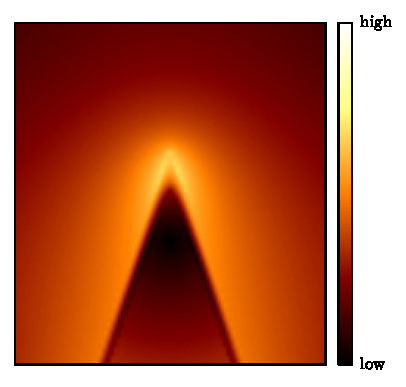
\includegraphics[width=\textwidth]{figures/lightning_rod_effect}
\vspace{-25pt}
\caption[Calculated magnitude of the electric field around a tip showing the lightning rod effect]{\textbf{Calculated magnitude of the electric field around a tip showing the lightning rod effect.} Compression of the field lines around the sharp corner of an equipotential surface leads to a localised, non-resonant field enhancement.%
\footnote{Poisson's/Laplace's equation is solved for a tip structured electrode with a surface charge distribution separated by some distance from a planar metal counter electrode of the opposite surface charge.}}
\label{fig:lightning_rod_effect}
\end{wrapfigure}

The {\color{red}electromagnetic (near-field)} response of tips can be broken down into individual components that constitute the enhancement mechanism. The two main optical components are a lightning rod effect and a resonant plasmon contribution for metallic tips \cite{esteban2006, zhang2009, schmid2013}. The main focus of current tip work is to tune and optimise the plasmonic component, however progress in sharpening tips has led to increases in the lightning rod component. Both of these components are important to consider to understand and control the tip near-field.
Regardless of plasmonic behaviour, metallic tips intrinsically exhibit a lightning rod effect, instilling a non-resonant component of near-field enhancement under the application of an applied field. From the definition of the electric field $\vec{E}(\vec{r}) = -\vec{\nabla} \phi(\vec{r})$ it becomes apparent that the electric field is strongly dependent on geometry with field lines perpendicular to the equipotential conductor surface. The more curved a surface, the more compressed the field lines become around its surface due to accumulation of surface charge.
This can be described by $E = \sigma/\varepsilon_0$ where $\sigma = q/4\pi r^2$ and $r$ is the radius of curvature. Since $E \propto 1/r^2$ the electric field is larger in regions of smaller  curvature. This effect is shown using a simple sharp tip model in \figurename~\ref{fig:lightning_rod_effect}.
Even without a plasmonic component sharp tips provide a promising platform for localised near-field enhancement.

% Experimental observation of characterisation of tip structures
%\begin{figure}[h]
%\centering
%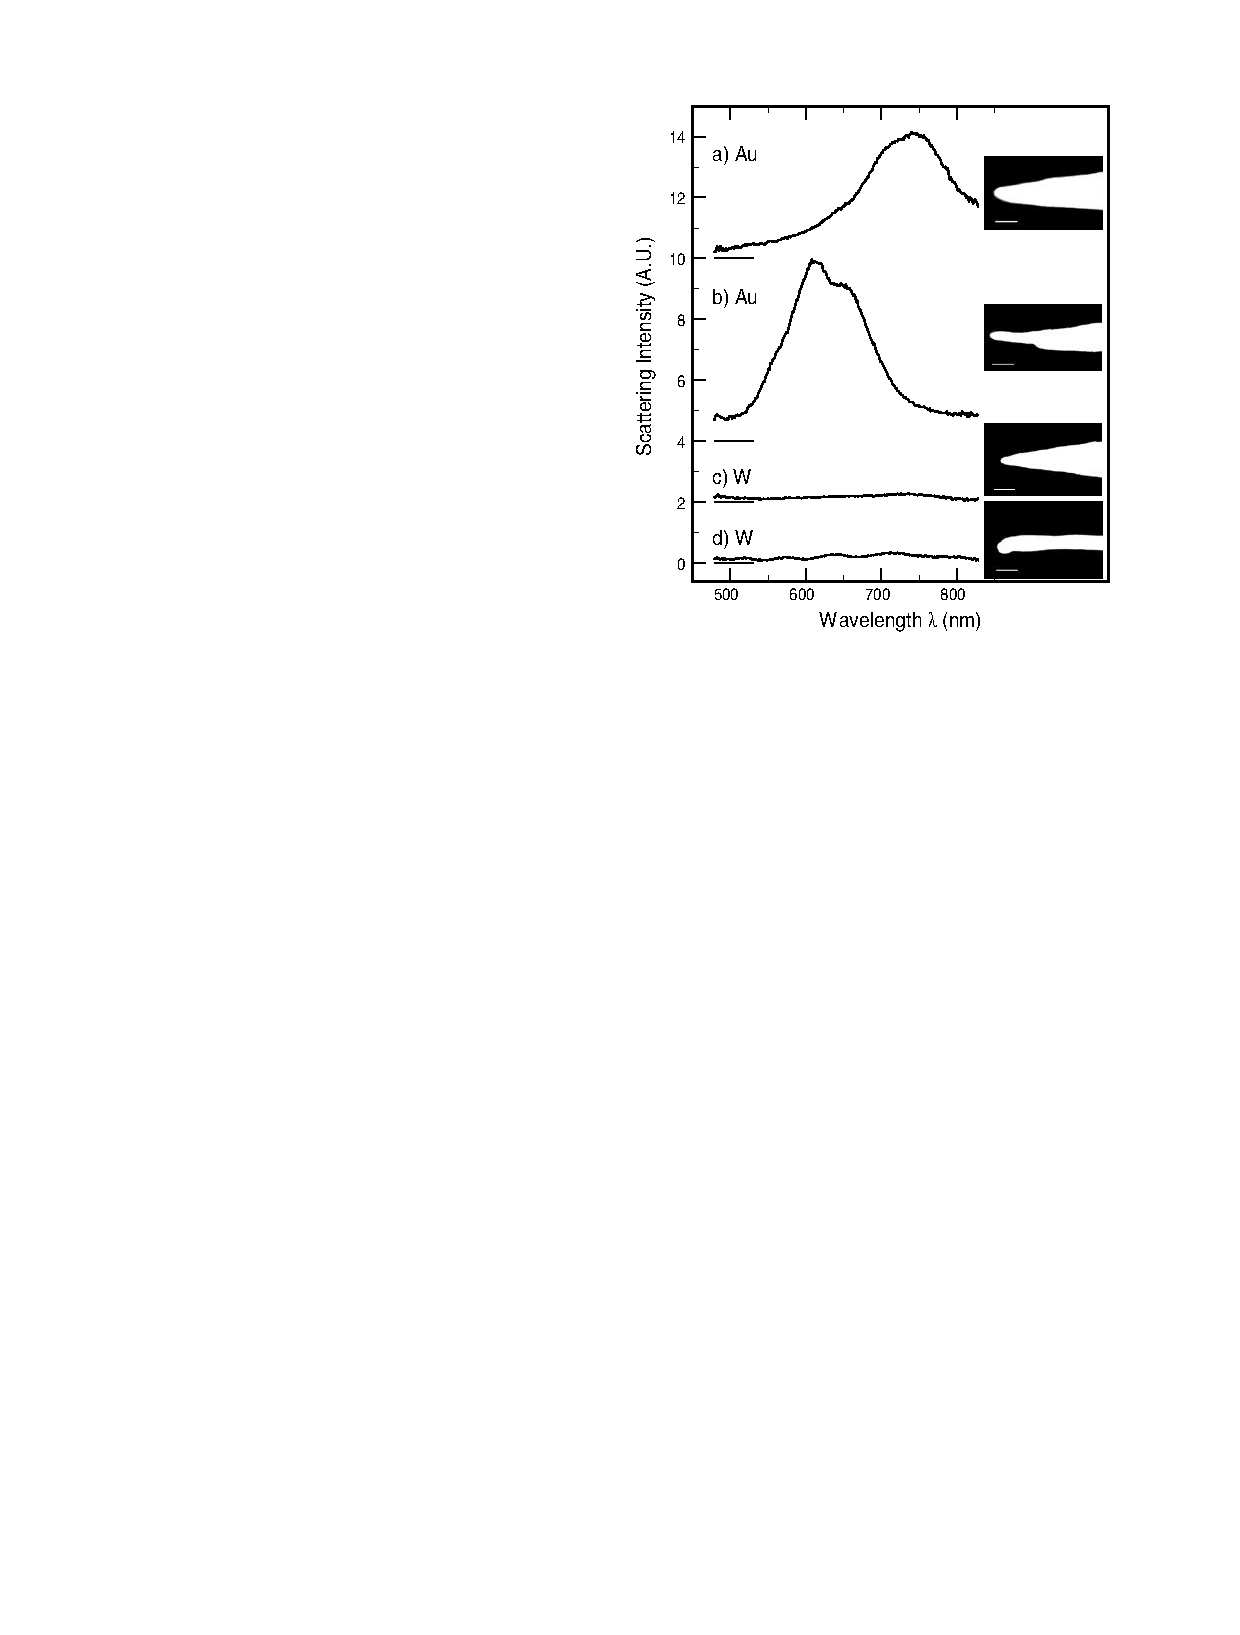
\includegraphics[width=0.3\textwidth]{figures/literature/neacsu2005b}~
%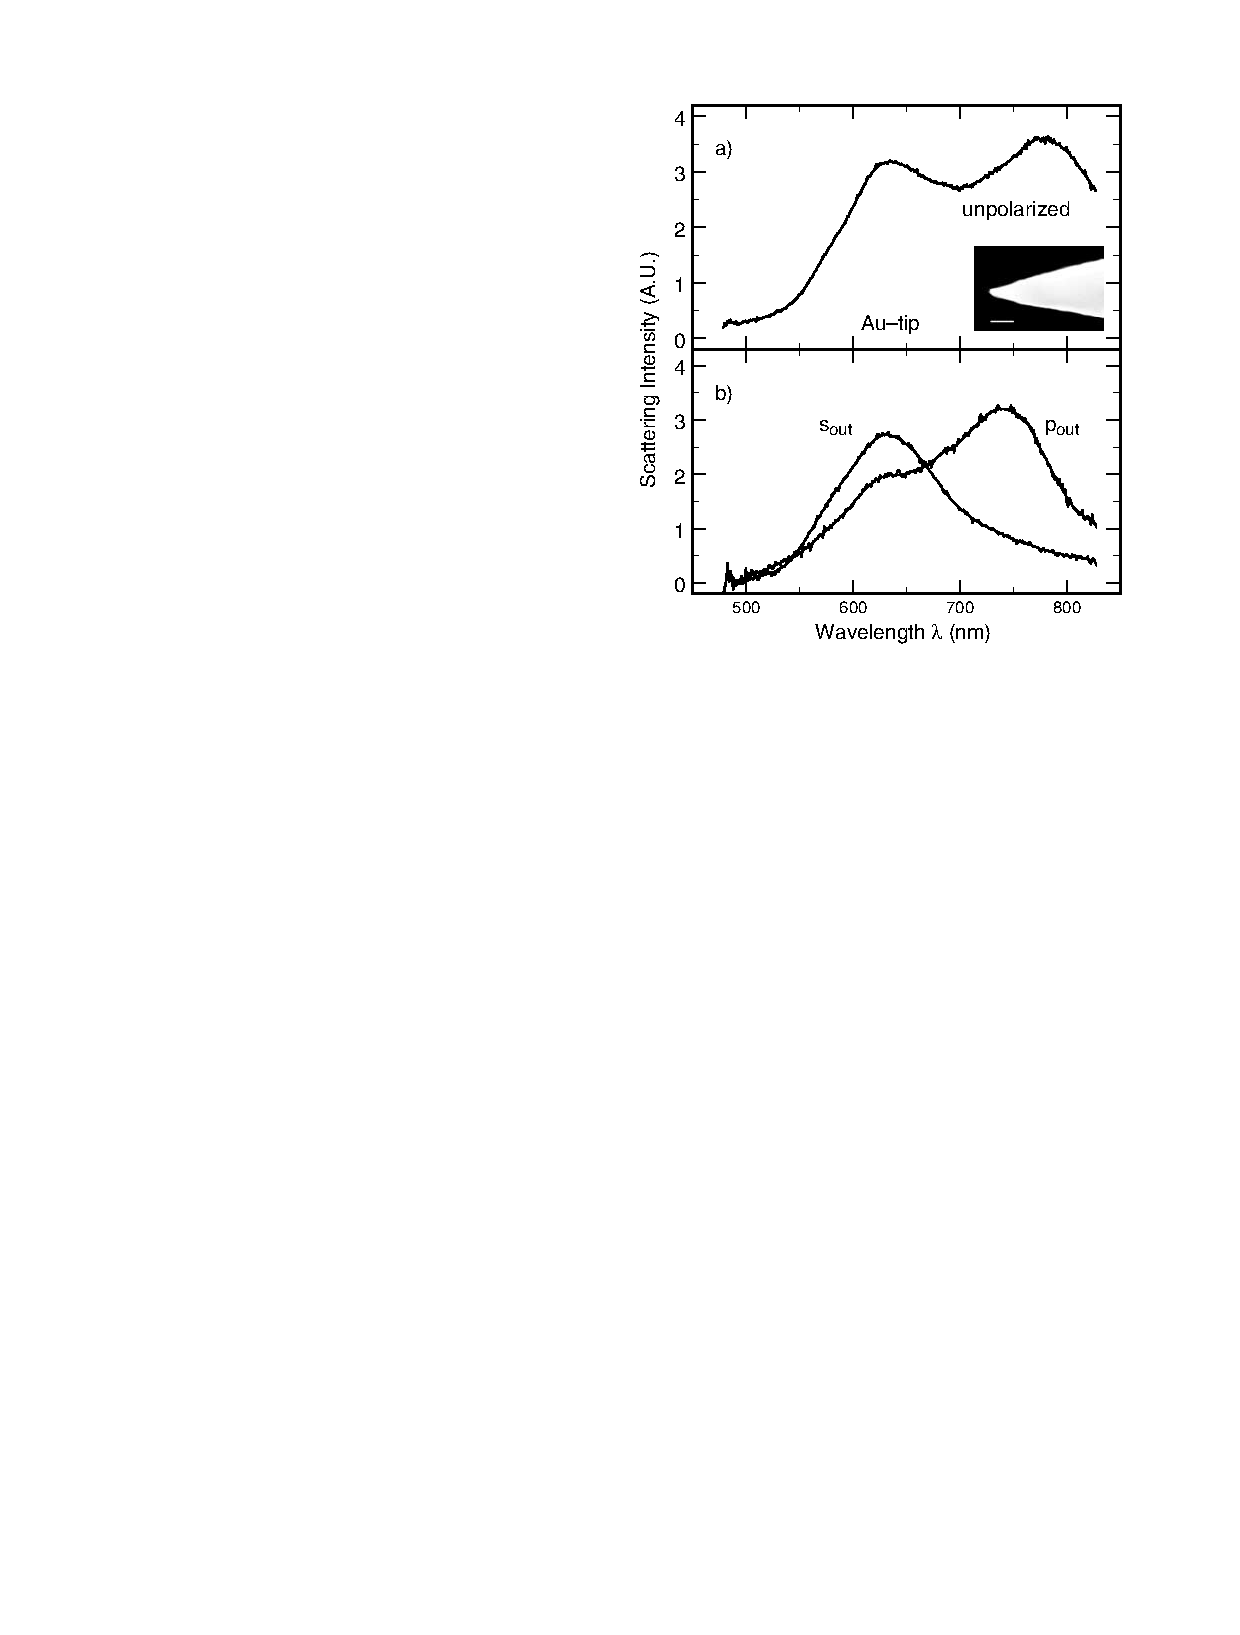
\includegraphics[width=0.3\textwidth]{figures/literature/neacsu2005c}
%\caption[Initial near-field scattering spectra of Au and W tips \cite{neacsu2005}]{\textbf{Initial near-field scattering spectra of Au and W tips \cite{neacsu2005}.} Resonances in scattering spectra for Au (left) are associated with SPP excitation at the tip apex. W tips show no similar resonances. Due to the anisotropic nature of the tip geometry there is a polarisation dependence to resonances (right).}
%\label{fig:neacsu2005}
%\end{figure}

% The plasmonic component
The expected plasmonic component arises from the curvature of the metal-dielectric interface at the tip apex. This allows for either the excitation SPPs are the apex or for SPPs propagating towards the apex to localise due to {\color{red}adiabatic nanofocussing \cite{}}.
The first direct observation of plasmons in tips was in 2005. Scattering of evanescent waves at the surface of a prism by a tip was used to measure the near-field response in Au tips \cite{neacsu2005}. The 600--\SI{800}{nm} spectral resonance present in Au, but not W, was attributed to excitation of SPPs at the tip apex. %Polarisation dependence showed that...
% \cite{Neacsu2006} also shows spectrum and image coupling
Further independent measurements of evanescent field scattering showed similar results \cite{mehtani2006}. $\sim$75--\SI{100}{nm} shifts were observed between Ag and Au tips with a \ce{Si3N4} base tip redshifting the resonances $\sim$\SI{30}{nm} compared with coated W tips with TERS measurements suggesting that enhancement correlated with the position of the spectral resonance.

LSP excitation proves more difficult due to the extended size of the typical tip structure ($\sim$\SI{20}{\micro\metre}). Simulations of shorter tip geometries show visible to NIR LSP resonances, however these redshift and diminish with increasing tip length \cite{zhang2009, huber2014}. It's for this reason that the standard metallic tip geometry makes for a poor optical antenna.
{\color{red}To date, despite these measurements, there is little work done to understand the optical response of tips and to characterise tips before applying them for near-field enhancement.}

% Design of TERS microscopes
\begin{wrapfigure}{O}{0.6\textwidth}
\centering
\vspace{-10pt}
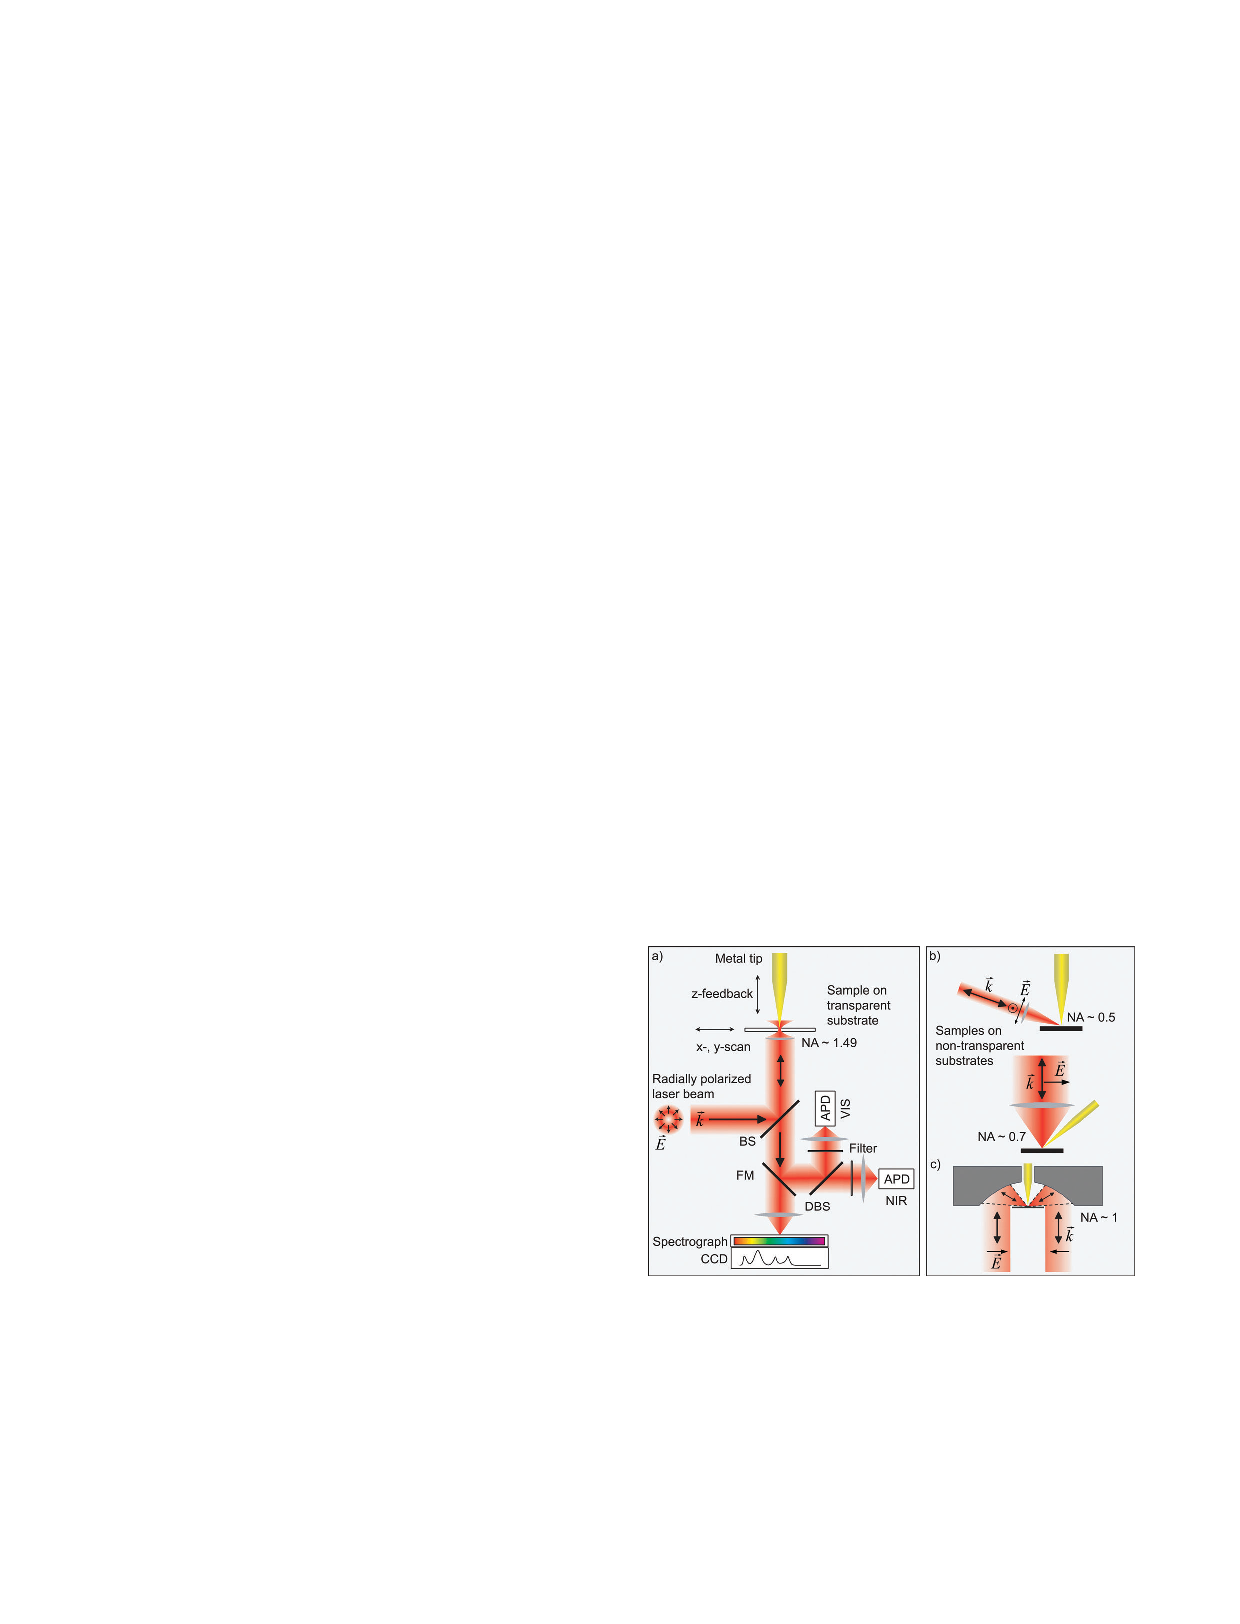
\includegraphics[width=\textwidth]{figures/literature/mauser2014a}
\caption[Typical optical geometries found in TENOM experiments \cite{mauser2014}]{\textbf{Typical optical geometries found in TENOM experiments \cite{mauser2014}.} The most prominent system is the bottom-illumination/back-illumination configuration utilising high-NA objectives. The other main geometry is the side-illumination configuration.}
\label{fig:ters_geometries}
\end{wrapfigure}

Since initial investigations, tip-based systems have been designed in two configurations: the side-illumination configuration and the bottom-illumination configuration. Both configurations are shown in \figurename~\ref{fig:ters_geometries}. The specific design of a TENOM microscope is important as it defines the collection and, more importantly, excitation geometries for the tip.
% Side-illumination
% zhang2013 - Ag tip on Ag(111) surface
% wickramasinghe2014 - Au tip with stimulated Raman
Side-illumination has been used successfully in a number of cases \cite{mehtani2006, zhang2013, wickramasinghe2014} but suffers generally from far-field scattering overshadowing the near-field scatter. This requires more complex optical geometries to fix, such as using polarisation-resolved approaches.
% Bottom-illumination
% hayazawa2001 - Ag tip on Ag surface, 
% uetsuki2012 - Au tip on Au(111) surface, 642 nm, EF=1e7
The dominant microscope design is the bottom-illumination configuration using a $\mathit{NA}>1$ objective to illuminate the tip evanescently using a mask in $k$-space. Masks are similar to regular dark-field microscopy except that only $\mathit{NA}>1$ light is transmitted. This approach means minimal scattering background due to total internal reflection (TIR) of the incident light with only near-field scattering collected through the $\mathit{NA}<1$ aperture. While many use this single objective system \cite{hayazawa2001, yeo2006, yeo2007, zhang2013experimental, kumar2014} other use a secondary low-NA side-collection objective \cite{uetsuki2012}. Bottom-illumination has the advantage that its evanescent wave illumination has the capability to couple to surface plasmons in both the sample and the tip once it is within the near-field. At this point coupling between a metallic tip and metallic sample can also occur, forming a hot spot. The disadvantage of using bottom-illumination is that it requires transparent samples (or thin enough to transmit some light) mounted onto a reflective, planar surface, which is not always possible.

\subsection{Challenges associated with Tip-based Near-Field Microscopy}

\begin{figure}
\centering
\fcapside[\FBwidth]
{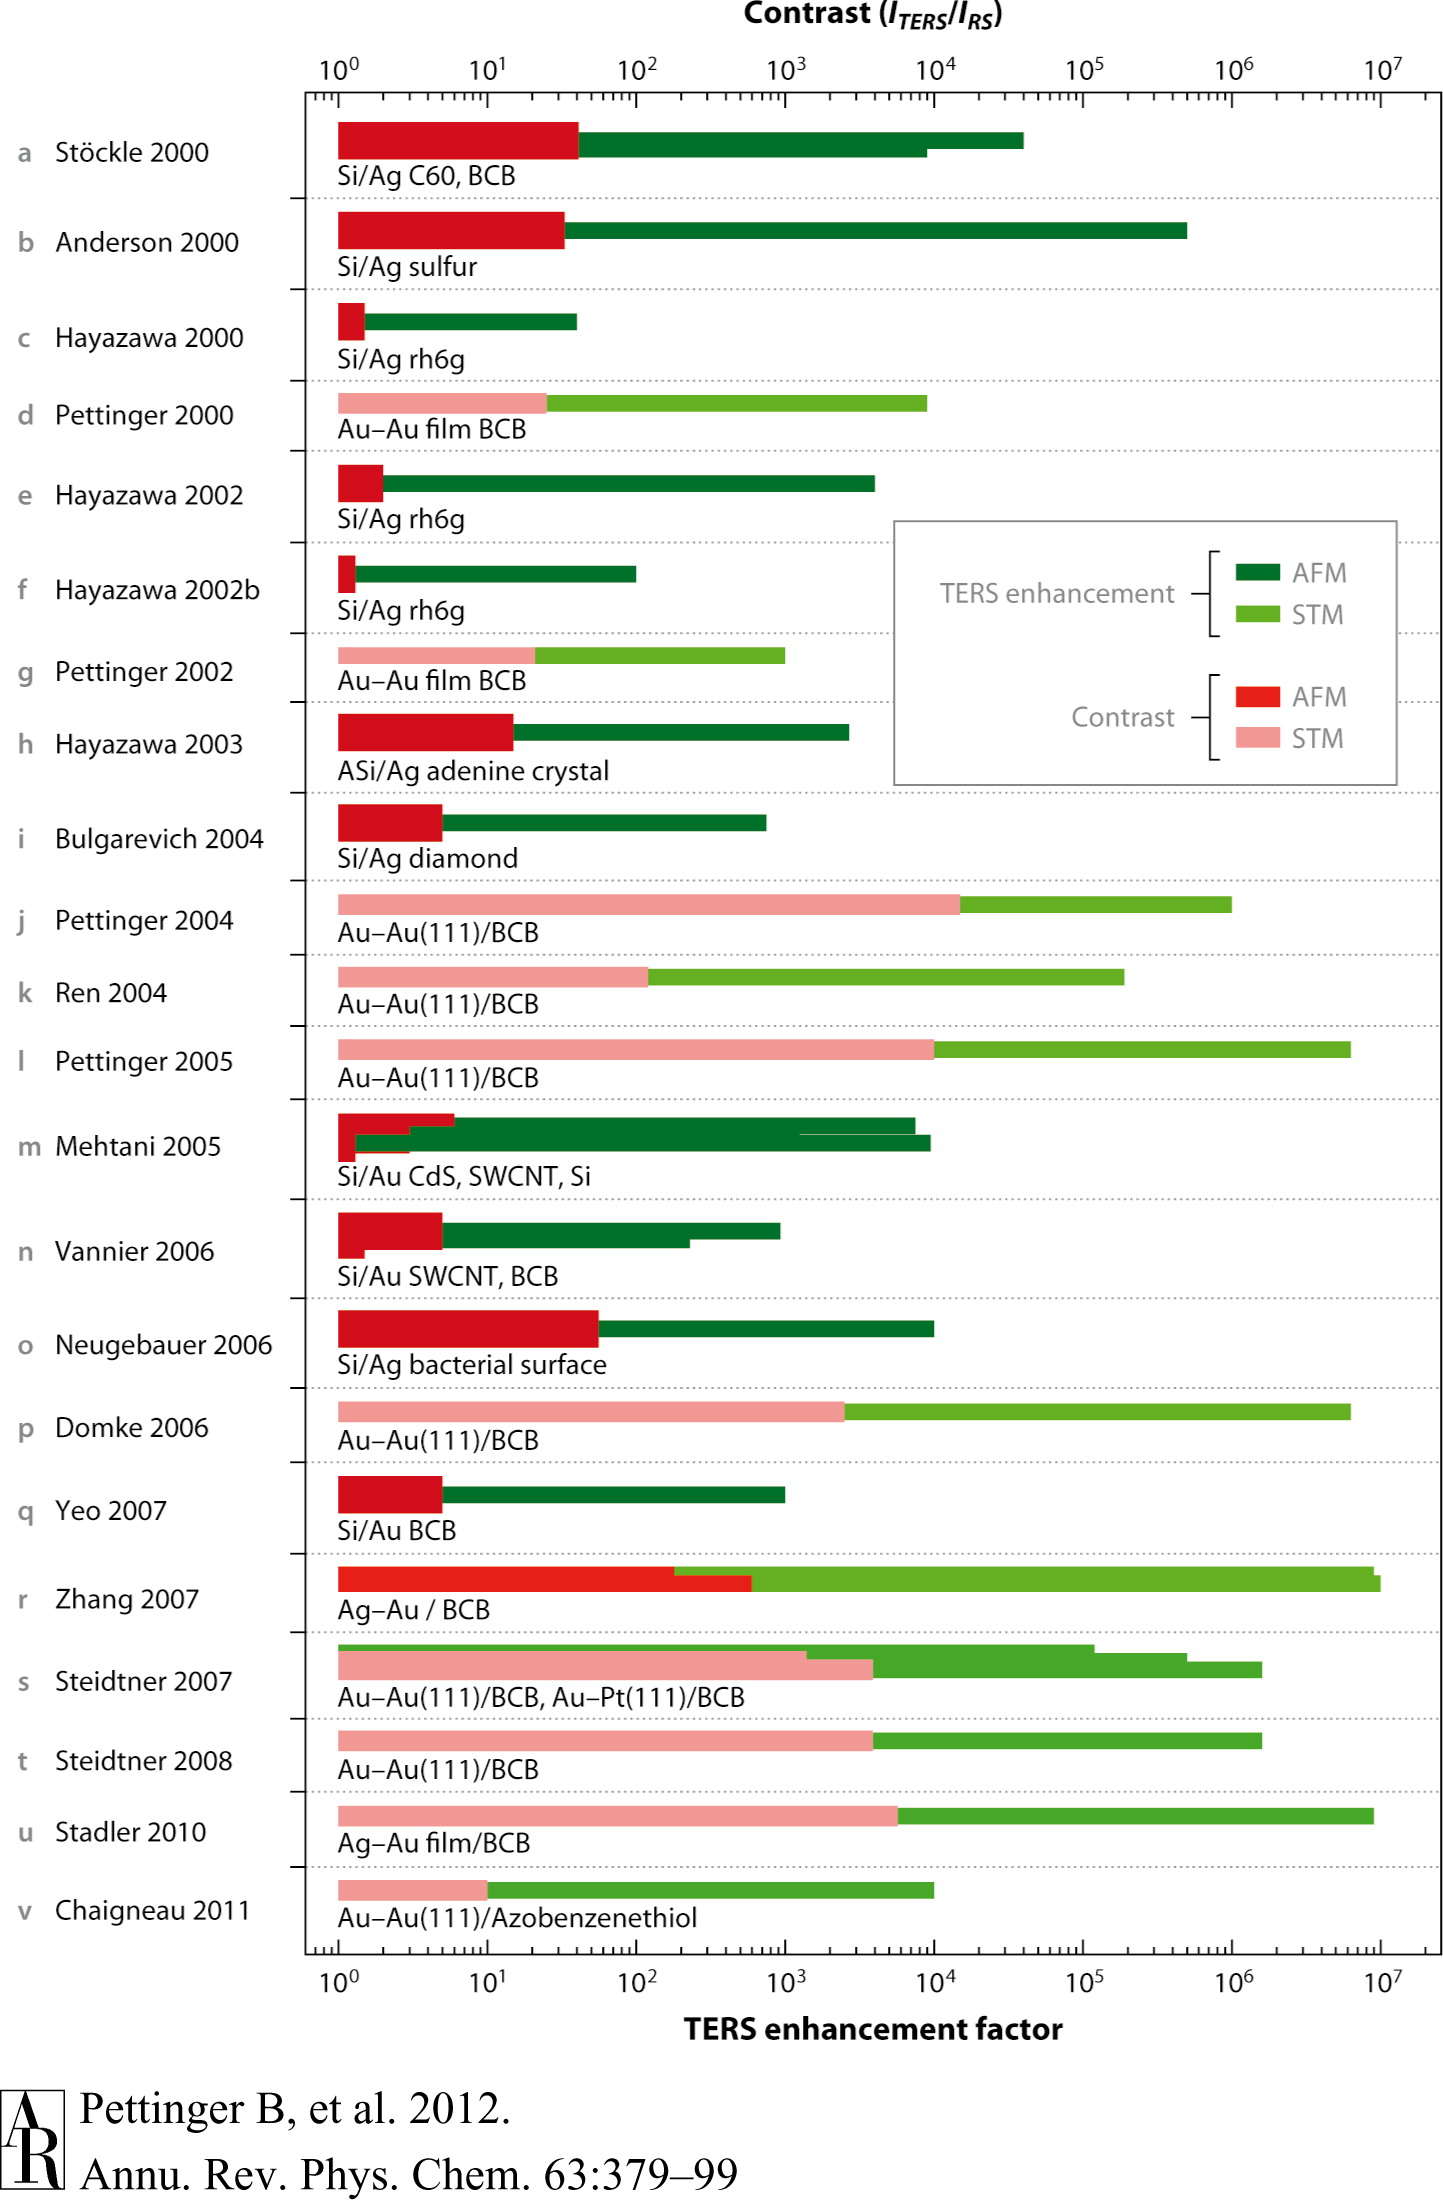
\includegraphics[width=0.7\textwidth, clip=true, trim=0 35 0 0]{figures/literature/pc630379_f8}}
{\caption[Comparison of TERS field enhancements and contrasts reported between 2000 and 2011 \cite{pettinger2012}]{\textbf{Comparison of TERS field enhancements and contrasts reported between 2000 and 2011 \cite{pettinger2012}.} STM tips, likely due to their increased sharpness, outperform AFM tips. Ag tips outperform Au tips. Larger enhancements are observed in systems where there is an underlying thin, noble metallic film. Statistical correlations still remain somewhat weak, showing the current variability in TERS experiments, attributed to irreproducibility of enhancing tips.}
\label{fig:pettinger2012}}
\end{figure}

% Challenges for TERS and comparison between measurements
Since the initial measurements of tip plasmons, techniques such as TERS and a-SNOM have become widespread and generally accepted. However, they are currently not reliable enough to be considered as a standard technique.
The current challenges with tip-based techniques include improving the reproducibility of the near-field enhancement between tips \cite{blum2014, kumar2014}, successful modelling of the optical processes and understanding the optical response of tips \cite{}.
Lack of control of the tip near-field is both a result of the irreproducibility of the tip geometry and the {\color{red}lesser} understanding of the optical processes, leading to large variations between reported field enhancements. A selection of TERS field enhancements and contrasts from reports between 2000 and 2011 showing the large variability are shown in \figurename~\ref{fig:pettinger2012}.

% Sharpness and lightning rod effects
It is clear that sharper STM tips result in a larger field enhancement than AFM tips. Comparative studies have also shown similar trends \cite{raschke2003}. This is most likely evidence that the lightning rod effect plays a significant role in the near-field enhancement process. Intuition suggests that the sharper profile of solid metallic STM tips means a larger lightning rod component compared with metallised AFM tips. Studies have also shown that large enhancement factors can be reported due to non-plasmonic artefacts caused by the tip shaft \cite{ramos2012}. These artefacts can be removed to recover the near-field enhancement \cite{kumar2014} {\color{red}(noting that lightning rod effect is still a near-field enhancement)}, therefore the possibility for a plasmonic response is not ruled out.

% Plasmonic component
\begin{figure}
\centering
\caption[]{\textbf{SEM images of metallised tips showing the granular texture and apex sharpness.} (a)\cite{hayazawa2001, hayazawa2012}.}
\label{fig:metallised_tips}
\end{figure}

% Morphology dependence
Variability between similar measurements is not solely due to differences in experimental setup or a change in tip sharpness, as discussed before. A large amount of variability stems from the surface metal morphology.
The plasmonic component of the tip is generally reported to originate from surface roughness that mimics the optical antenna properties of nanoparticles. Each grain of the coating can act as points at which plasmons can couple or radiate, hence a grain located at the apex can plasmonically enhance the near-field. For this reason TERS tips are typically metallised dielectric tips, coating using evaporation under similar conditions used to deposit metal islands on film \cite{hayazawa2001, hayazawa2012} or chemical reactions \cite{bailo2008}.
Orientation of the tip with respect to the sample has also been shown to influence the near-field enhancement \cite{yeo2006}.

% Material dependence
As with conventional plasmonics, Ag tips generally outperform Au tips under visible light, though these claims strongly depend on the underlying tip material and the morphology of the metallic surface used in the experiment. Plasmon excitation is complicated as resonances are shifted by the refractive index of the underlying tip material. Careful consideration must be given when pairing a TERS probe with a laser. Experiments have demonstrated that matching the excitation wavelength to the plasmon resonance increases the near-field enhancement \cite{yeo2006, yeo2007, cui2007, hayazawa2012}. Numerical simulations further show that resonance positions are highly sensitive to the metallic coating thickness when below the skin depth ($\sim\SI{40}{nm}$), suggesting some experimental variability comes from the accuracy of the metallic deposition process \cite{huber2014}.

The previous observations all supports the hypothesis that a tip in some ways supports plasmons, which contribute to the overall near-field enhancement. However, the dependence on random depositions of rough metal is the main downfall of TERS and the more likely reason for the lack of reproducibility between measurements. Though many reports are motivated by the need to improve the reproducibility, typically via tuning the underlying tip dielectric material, very few have achieved this due to the reliance on the grain structure.
\cite{blum2014}

Larger enhancements also occur when a thin metallic substrate films is used, suggesting formation of more localised gap plasmons.%
\footnote{Should probably look into those references and append wavelengths.}
Even between similar measurements there is a strong variability. Variations can be attributed to many factors other than the enhancement from the tip, including the tip placement, optical setup and illumination/collection geometry used.
As tips are rarely characterised there is little traceability between measurements from which to determine any relevant cause for difference. However, in this time, further experiments have been carried out to study the plasmonic nature of noble metal tips to understand the near-field around an illuminated tip. Theory has also been developing to complement experiments and successfully model and disentangle the optical response of tip systems.

% Gap mode formation
Gap modes may form in tip systems where the underlying sample substrate is metallic. Coupling between a tip and excited SPPs on the planar metallic substrate yields a hot spot with potentially large enhancements. This is often exploited and, as a result, the Raman enhancement has been shown to rise to the order of \num{e7} when illumination is on resonance with the gap mode\cite{uetsuki2012}. % maybe comment more on the mechanism for this excitation as side illumination alone may not be enough i.e. excitation geometry more important than collection.

% Electrical excitation
Since tips are typically illuminated with single wavelength light it becomes difficult to discern plasmonic features hidden in the collected light. Electrical excitation of plasmons has been used to circumvent this limitation after the observation of light generation between a STM tip and a metal surface \cite{}. Electrical excitation functions to both remove the background light from the illumination source and also can excite any modes with frequencies $\nu$ satisfying $h\nu \leq eV$, where $V$ is the surface voltage of the STM. Using tunnelling current excitation, light has been observed from both the tip-air-metal surface gap \cite{} and the interface between the metal surface and its underlying dielectric substrate \cite{wang2011}. Light detected from metal-glass interfaces is leakage radiation from SPPs on the metal-air interface as the SPP dispersion crosses the light line ($k_{SPP} = k_{glass} = nk_{air}$, see Figure.~\ref{fig:spp_dispersion}, chapter \ref{ch:theory}) \cite{wang2011}. Since light cannot leak from SPPs at the metal-air interface the detected light must be from gap plasmons between the tip apex and the surface \cite{}. It is thought that 95\% of the emission is due to SPP excitation rather than LSP excitation \cite{wang2011}.
% this causes problems with the idea of antenna modes.

%\begin{figure}
%\centering
%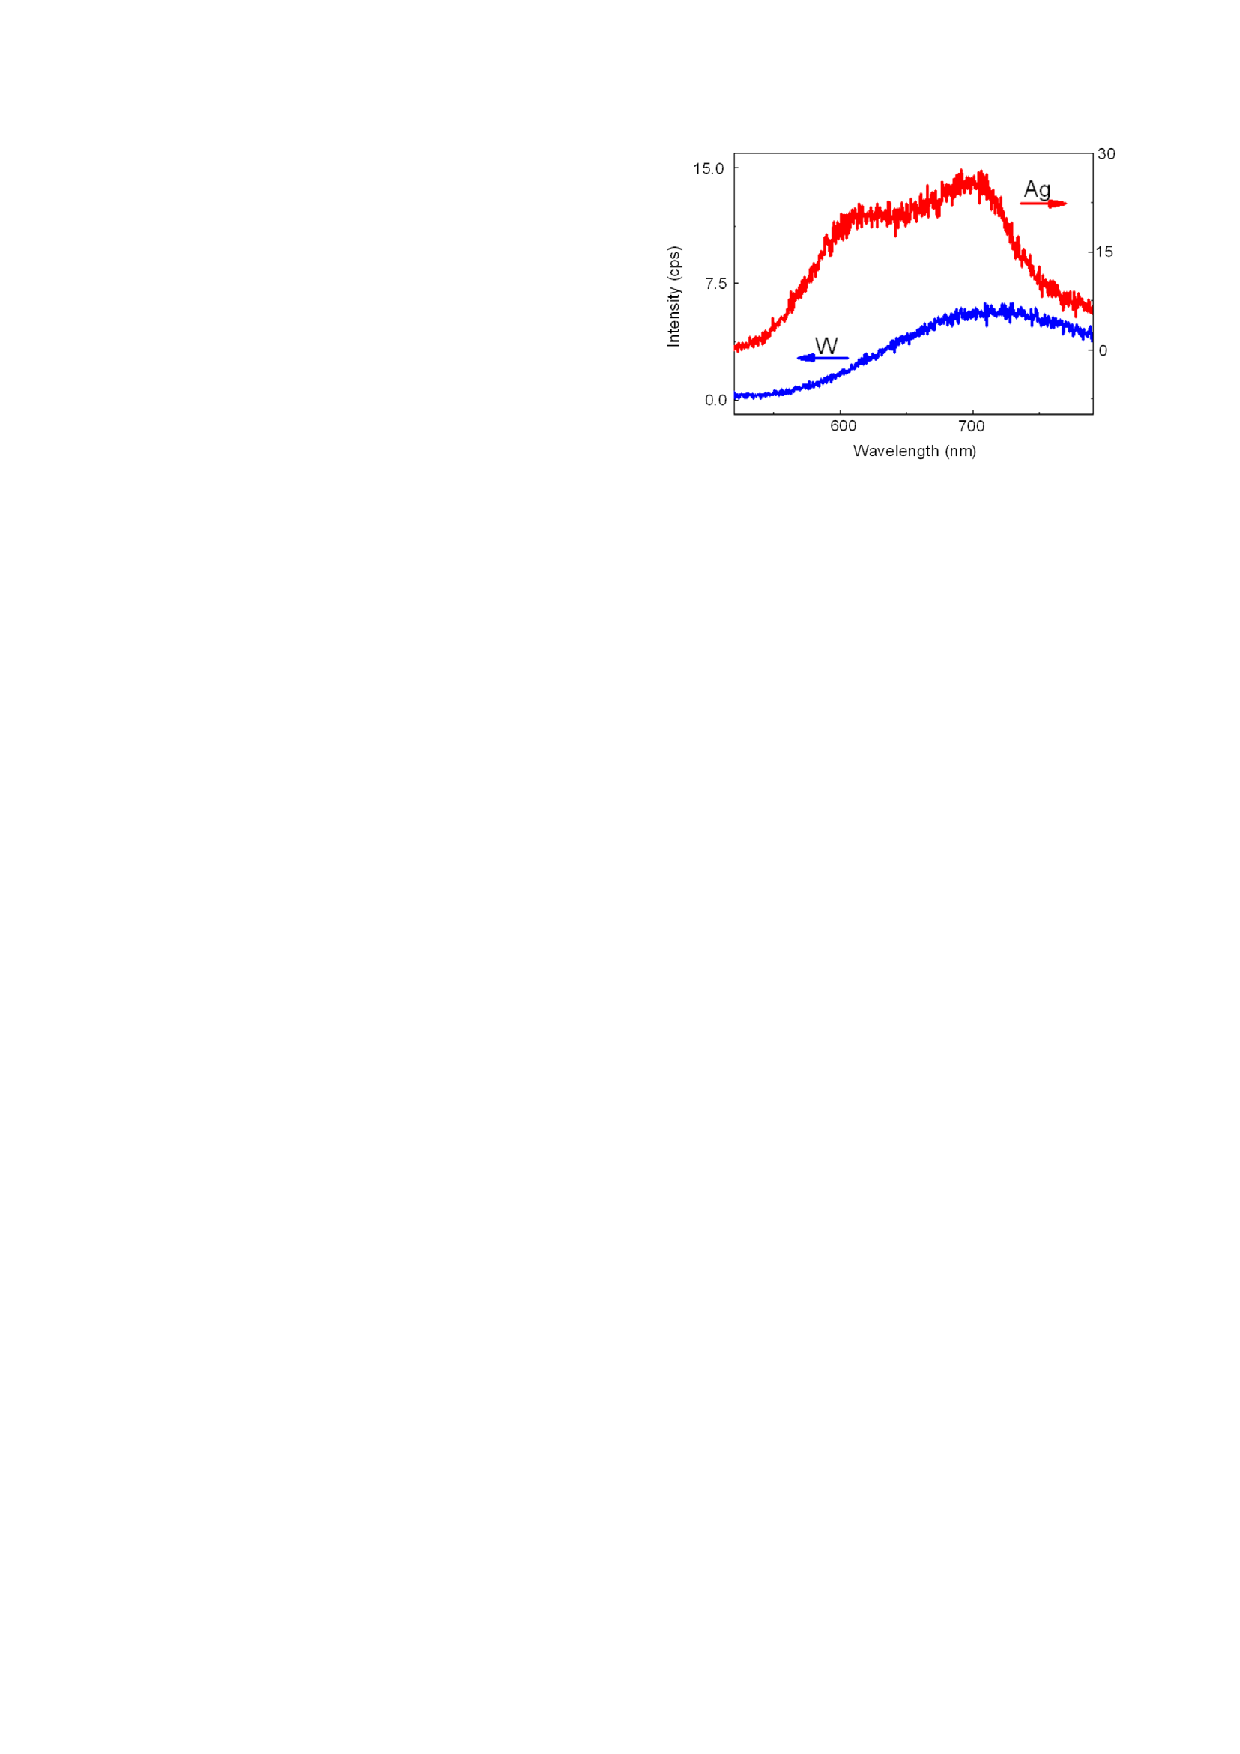
\includegraphics[width=0.5\textwidth]{figures/literature/wang2011}
%\caption{Emission spectra from W (blue) and Ag (red) tip-air-Au surface tunnelling gaps \cite{wang2011}. The spectrum of W is explained by $h\nu_{photon}<eV$ while the spectrum of Ag is reminiscent of a \SI{60}{nm} AgNP on Au spectrum.}
%\label{fig:wang2011}
%\end{figure}

\cite{taguchi2009}

{\color{red}
\subsection{Experimental Considerations for Tip-Enhanced Near-Field Measurements}
While it is accepted that tip-based field enhancement is a working phenomenon, many are content to apply this knowledge and focus on improving the equipment and imaging procedures in order to maximise the quality of near-field images. Mostly this is in regard to the removal of background scatter.
The use of lock-in detection of a vibrating AFM cantilever has been successful in isolating the signal when the tip is near to the sample compared with the general background scatter of the tip and sample is the laser focus \cite{}. Other solutions are to remove the background scatter altogether by fabricating tips with side gratings in order to couple light into propagating SPPs that focus and reradiate at the apex to form a nanoscale light source \cite{}. These reports also demonstrate that a sharp apex acts as a defect point at which SPPs can outcouple to photons. By reciprocity it also means that near-field light can also excite SPPs at the apex which can propagate away from the apex.}

% Reiterate why this means tips need better characterisation and understanding
For this reason a selection of techniques are desired to optically characterise tips prior to use.

\subsection{Optical Antenna Tips}

% Transitioning the discussion from sharp to nanostructured tips
The mode mismatch caused by the size difference between diffraction-limited light and the nm-scale results in a 3--4 order magnitude coupling efficiency loss \cite{berweger2010}. As described previously, a plasmon acts as an optical antenna. A good optical antenna has the ability to effectively modify the density of electromagnetic states such that the far-field radiation impedance is efficiently matched with the impedance of a near-field evanescent mode and vice versa \cite{novotny2006, novotny2011}. The antenna opens up scattering pathways that connect wave states ($k$-vectors) by creating new intermediate states, thus enabling local evanescent waves to find a pathway to radiative emission. Metallic tips, in their standard form, are not particularly good optical antennae \cite{zhang2009}.
{\color{red}The lack of radiative lower order multipolar resonances greatly diminishes the radiative cross section \cite{renger2004}.}
To improve transmission efficiency, standard sharp, pointed tips and their surrounding structures can be modified or nanostructured to introduce such intermediary states which effectively couple the far-field to the near-field \cite{mauser2014}.

% Nanoantennae tips
\begin{figure}%{wrapfigure}{O}{0.5\textwidth}
\centering
%\vspace{-10pt}
%\fcapside[\FBwidth]
{
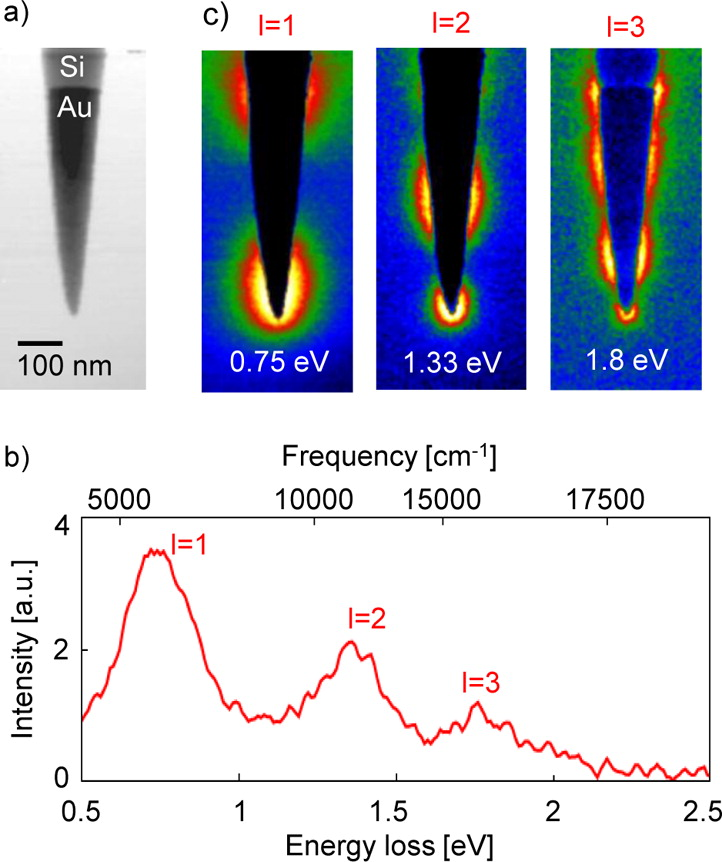
\includegraphics[width=0.45\textwidth]{figures/literature/nl-2012-04289g_0003}
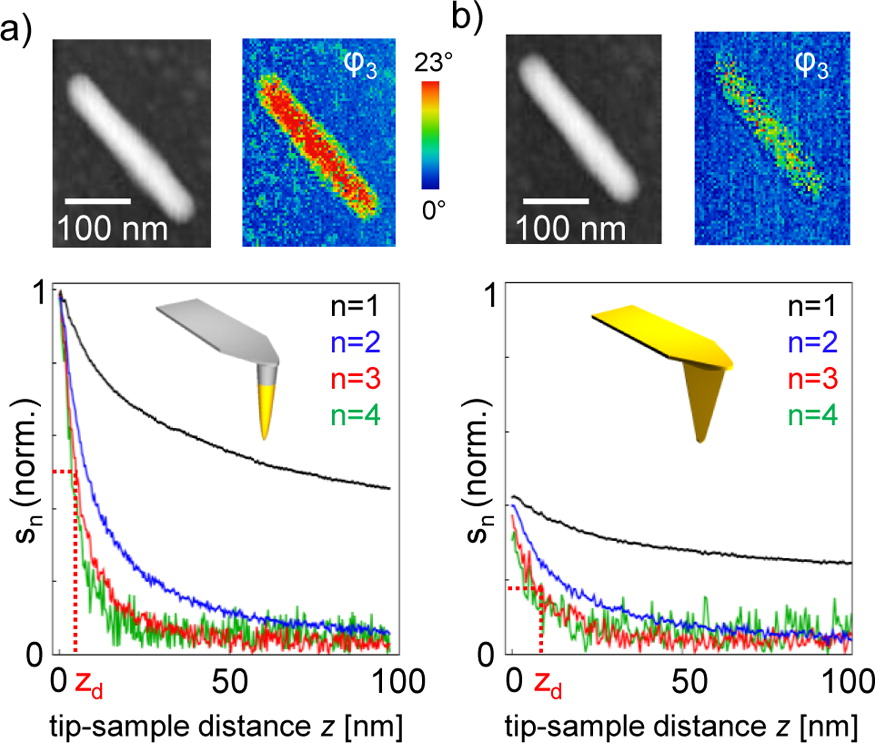
\includegraphics[width=0.45\textwidth]{figures/literature/nl-2012-04289g_0009}
}
%\vspace{-15pt}
{\caption[Comparison between standard Au and nano-antenna AFM tips \cite{huth2013}]{\textbf{Comparison between standard Au and nano-antenna AFM tips \cite{huth2013}.} Nano-antenna tips comprise a Au nanotip on a FIB-cut Si AFM tip. EELS spectra show multipolar rod LSP plasmon modes and scattering measurements demonstrate that nano-antenna tips outperform standard metallised tips.}
\label{fig:huth2013}}
\end{figure}%{wrapfigure}

Designs in which the tip is removed and replaced with a planar bow-tie antenna \cite{weber2010} or nano-cone \cite{fleischer2011} have demonstrated improved field enhancements due to resonant excitation of a LSP mode in the modified apex structure. Such modification and attachment is typically carried out using FIB machining of base AFM tip structures during electron microscopy, in which the size of the structure can be varied to tune the plasmon resonance. Investigations into the plasmons of similar nano-tip optical antennae of different lengths show that scattering from the near-field is increased by 120\% when using resonant localised plasmon modes \cite{huth2013}. Note however that this is using a side-illumination geometry which is efficient only at targeting multi-polar antennae.

% Grating tips as nanoscale light sources
\begin{figure}
\centering
\fcapside[\FBwidth]
{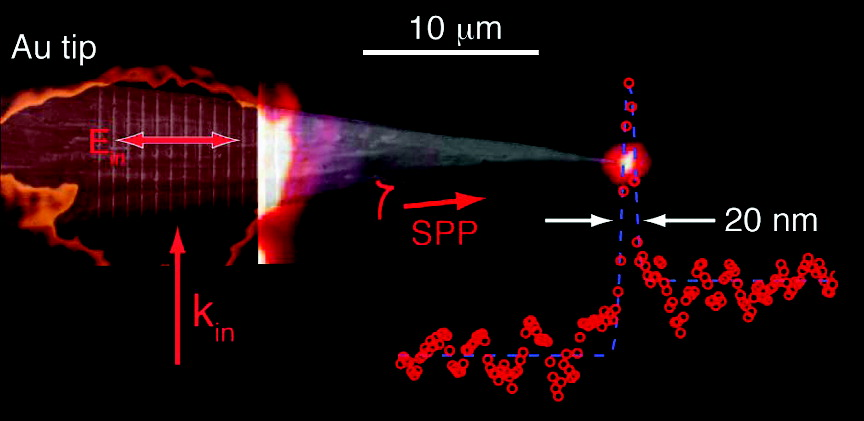
\includegraphics[width=0.5\textwidth]{figures/literature/nl-2009-03574a_0004}}
{\caption[A grating-coupled Nano-tip light source]{\textbf{A grating-coupled Nano-tip light source.} Imprinting a grating onto the side of an AFM tip allows far-field excitation of SPPs, which focus and localise at the apex, emitting nanoscale light \cite{neacsu2010}. This can be used to circumvent far-field background scatter at the apex for improved near-field measurements \cite{berweger2010, berweger2012}. Emission mechanics are similar to electrical excitation of SPPs but no longer requires an underlying plasmonic substrate and gap coupling.}
\label{fig:neacsu2010}}
\end{figure}

One particularly useful example of SPPs on the surface of tips and nanofocusing is illustrated by imprinting a grating onto the side of the tip \cite{neacsu2010} or by coupling to SPPs using a photonic crystal waveguide \cite{bek2011}. Usually near-field evanescent wave coupling is required to excite SPP modes in tips, however diffraction gratings also impart momentum allowing photons to couple with surface plasmons \cite{}. When the grating is illuminated excited SPPs  propagate towards the apex. Only a single mode can exist at the apex, which localises and re-emits as a nanoscale light source (Figure~\ref{fig:neacsu2010}). As with electrical excitation experiments, this clearly demonstrates that SPPs will radiate into the far-field at the apex of a sharp tip. Unlike electrical excitation, however, plasmonic gap coupling is not required to scatter SPP radiation. A disadvantage is that this technique is only shown as viable for $\lambda_{SPP}\geq\SI{800}{nm}$.
%From this observation it becomes clear that efficient coupling to excite SPPs is more important for nanophotonics than plasmonically outcoupling the scattered light.

Although nanostructuring has been shown to improve the optical response of tip structures the current techniques, mainly based on FIB techniques, are costly and time consuming. Part of this project is dedicated to the development of a simple method for producing plasmonic antenna tips.

\subsection{Theoretical Modelling of Tip Nanophotonics: Understanding the Near-Field Response}

%\cite{Demming2005, Rogov2013}

Theoretical analysis and modelling of tip structures is difficult. The main difficulty comes from the range of length scales of tip structures. The apex diameters of tips can easily be below \SI{50}{nm} while the overall tip length can extend to over \SI{20}{\micro\metre} with various feature sizes in between.

% effective particle approach
An early, and ultimately dissatisfying, model considered the apex radius and material composition as the only important parameters, approximating the apex as a sphere \cite{}. The fundamental issue with this approach is that a sphere has a back surface on which poles of lower order \gls{lsp} modes exist. Predictions of spectra therefore include antenna modes not compatible with a realistic tip geometry \cite{}. Later approaches used an elliptical particle to mimic the increasing sharpness of a tip \cite{}. In this case the polarisability is redefined as,
\begin{equation}
\alpha_i(\omega) = 4\pi a_1a_2a_3\frac{\dielectric-\epsdi}{3\epsdi+3L_i(\dielectric-\epsdi)},
\end{equation}
to include the geometrical factor,
\begin{equation}
L_i = \frac{a_1a_2a_3}{2}\int_0^\infty \frac{dq}{(a_i^2+q)\sqrt{(q+a_1^2)(q+a_2^2)(q+a_3^2)}}.
\end{equation}
The resonance condition is then changed to,
\begin{equation}
\real{\dielectric} = -\frac{1 - L_i}{L_i}\epsdi,
\end{equation}
therefore by decreasing the geometrical factor the resonance decreases from $-2\epsdi$. This corresponds to a decrease in the frequency and a redshifted plasmon. The longer the particle is the larger the redshift until the particle is large enough to no longer be considered plasmonic. Using this approach, strictly within the quasistatic regime, it becomes obvious why a long, sharp tip cannot sustain lower order, multipolar \gls{lsp} modes that couple with the far-field.

The different length scales associated with a large tip causes issues when using modelling techniques that split a surface into a mesh grid. Around the apex a fine mesh with sub-nm grid sizes is required to accurately solve Maxwell's equations on such a small feature size, however it is not computationally feasible to use this mesh size across the whole \si{\micro\metre} scale structure.
% tip model too small - does not take into account the extended structure
In many cases only the tip apex is modelled with a high resolution grid resulting in unphysical modes appearing due to SPP or LSP excitation due to actually modelling a sub-\si{\micro\metre} scale antenna structure, like a nanoparticle \cite{}, or even modelling the apex as a nanoparticle. Plasmons such as these are artefact of an artificially small nanostructure, caused by interference between waves propagating along a much smaller surface than is actually available or polar charge distributions that cannot exist if the length of the tip is increased due to charge cancellation by the appearance of positive ions.
% adaptive meshing and accounting somewhat for tip length
On the other hand, adaptive meshing can be used to take the extended tip structure into account whilst maintaining a finer grid around the apex curvature. The length of the tip, although increased, still contributes some SPP interference resulting in visible modes.

% real shape of the tip rarely taken into account
Calculations also rarely take into account the actual shape of experimental tip structures (typically created using an etching process along crystal planes), instead exploiting symmetry to improve the calculation time by modelling the tip as a perfect cone.
% taking into account the actual length of the tip
%\begin{figure}[h]
%\centering
%{\small
%\begin{lpic}{figures/literature/zhang2009(0.7)}
%	\lbl[l]{12, 60; (a) $r=\SI{20}{nm},\ \alpha=\SI{15}{\degree}$}
%	\lbl[l]{90, 60; (b) $l=\infty,\ \alpha=\SI{15}{\degree}$}
%	\lbl[l]{166, 60; (c) $l=\infty,\ r=\SI{20}{nm}$}
%\end{lpic}
%}
%\caption{Numerical simulations of the field enhancement at the apex of a sharp Ag tip subject to changes in cone length, apex radius and cone angle \cite{zhang2009}.}
%\label{fig:zhang2009}
%\end{figure}
When the length of a more realistic tip structure is taken into account the resonant plasmon modes reduce disappear into a smooth continuum \cite{zhang2009}. Between \SI{200}{nm} length and an infinite length a tip transitions between supporting low order LSPs, then higher order LSPs, followed by only weak SPPs. LSPs are supported only when the entire tip structure is comparable in size to the focus, allowing light to drive in-phase collective oscillations of the conduction electrons. As the tip becomes larger than the focus, and hence the illumination wavelength, phase retardation occurs and higher order LSP modes dominate. Once the tip becomes larger than the focus collective oscillations are no longer possible, leaving only LSPs concentrated at the apex surface and SPPs. The SPPs form the periodic response in the field enhancement before disappearing due to increasing losses when the tip length is increased further. The field enhancement inevitably rises smoothly and non-resonantly towards the IR due to only a lightning rod effect contribution being present. In this case the rise is caused by the longer wavelengths becoming larger than the apex radius or curvature, thereby creating an apparent increase in sharpness. To this extent, Zhang \emph{et. al.} suggest that the improvement in TERS over time is correlated with the availability of new technology to fabricate sharper metallic tips since SPPs remain weak and lossy allowing the lightning rod effect to dominate. Furthermore, Figure~\ref{fig:zhang2009}(b) shows that even a sharp tip with a \SI{10}{nm} radius cannot compete with the enhancements brought on by collective LSP excitation in a broader apex.

Due to limitations in experimental fabrication processes the metallic surfaces can rarely be considered flat, with granular surfaces and atomic scale roughness considerably changing the plasmonic response \cite{}.

% discuss some simulations
Calculations of a Au tip approaching a Au surface, considering only the apex region (adaptive meshing), in the quasi-static approximation \cite{behr2008}. By considering only the quasistatic regime the Laplace equation can be analytically solved, simplifying the computation time and giving greater insight into the physical quantities and how they behave. However, this approach assumes a plasmon exists at the apex with no method of optical excitation other than evanescent wave coupling.

One difficulty when comparing a calculated near-field response compared with a measured far-field spectrum is distinguishing between modes which can exist but are dark and those which can couple with light, specifically considering what conditions are required for optical coupling. To this extent an antenna mode is applied to attempt to disentangle spectral modes into those which can be observed in the far-field and those which can't.

Despite the experimental drive to produce sharper tips, it has been suggested that the sharpness of tips eventually enter a regime where non-locality (quantum mechanics and electron-electron interactions) becomes important. In this regime the field enhancement is reduced and limited by nonlocal effects and localisation effects of structural surface imperfections and sharpness are heavily reduced \cite{wiener2012}, suggesting a quantum limit to field confinement.
{\color{red}Both the strength of the lightning rod effect and the confinement of SPPs are therefore limited, meaning that contributions from different plasmonic mechanisms is necessary to further pursue larger field enhancements with tips.}

{\color{red}Despite using an apex-localised, quasi-static model to analytically predict the spectral response of tips and tip-sample interactions, a visible frequency plasmon resonance ($\sim\SI{550}{nm}$) is calculated for a hyperbolic tip, one which is independent of cone angle, which only affects the field enhancement, but sensitive to tip radius (redshifts with decreasing radius) and gap coupling with a planar surface \cite{behr2008}. As with any quasi-static model phase retardation is neglected meaning it is not possible to predict multipolar resonances. While this model shows agreement with FTDT calculations \cite{} and early experimental measurements \cite{neacsu2005} the specific conditions required to excite the LSP are not discussed.

Experimental observations show that sharper STM tips give more enhancement than AFM tips \cite{yeo2006, pettinger2012}, suggesting that a significant component of tip enhancement is a strong contribution from the lightning rod effect. Simulations using the premise of an infinite conical tip computationally replicate this behaviour as the tip length is increased \cite{zhang2009}.}

%\begin{figure}
%\centering
%\caption{Comparison between metallised Au tips and Au antenna tips from EELS spectra and TERS measurements \cite{huth2013}.}
%\label{fig:huth2013}
%\end{figure}

Further evidence for the lack of a plasmonic contribution comes from the comparison between metallised Au tips and Au antenna tips \cite{huth2013}.

\FloatBarrier
\subsection{Plasmons in Apex-Nanostructured Tips}

%\cite{Fleischer2011, Denisyuk2012, Goncharenko2006, zou2009, lindquist2013}

% Introduction to nanostructuring
Recently, nanostructuring of the tip apex has been applied to tune and optimise the optical (plasmonic) properties of nanotips. By reducing the characteristic size of the apex structure, thereby giving it a new, more localised, geometry, light can be more strongly confined in more localised plasmon oscillations, hence the optical antenna properties of a nanotip can be substantially improved. The emergence of new plasmon modes unsupported by regular sharp tips then opens up new mechanisms through which light can be channelled to the nm-scale, such as direct far-field illumination.

% Spherical nanostructuring
The simplest geometry to impart onto a tip apex is a sphere. By doing so the tip gains plasmon modes similar to that of an isolated spherical nanoparticle. The specific mode depends on the method used for attachment as the base tip structure affects the plasmons. To date there have been a number of methods reported for spherically structuring a tip apex.

\begin{figure}
\centering
%\fcapside[\FBwidth]
{\begin{subfigure}[t]{0.35\textwidth}
	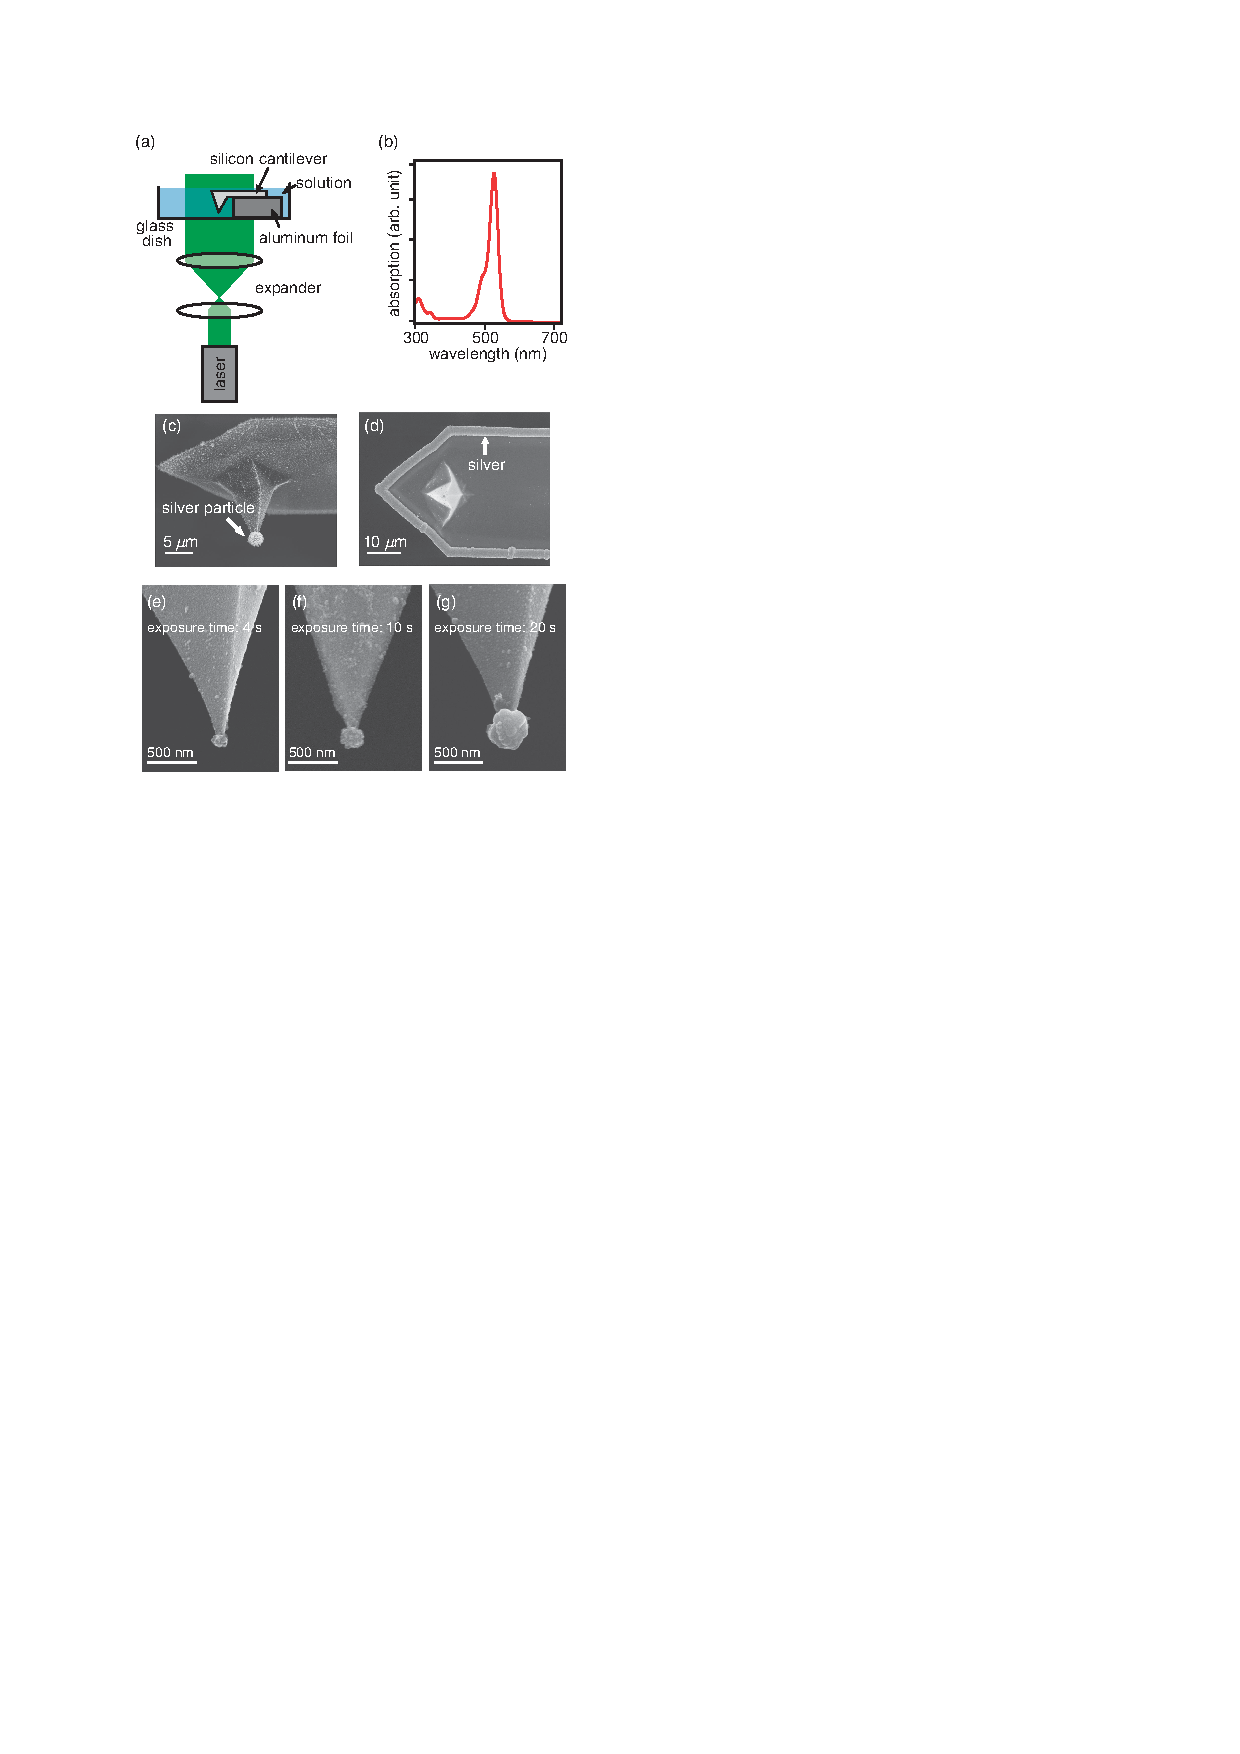
\includegraphics[width=\textwidth, clip=true, trim=0 0 0 130]{figures/literature/umakoshi2012a}
	\caption{Photochemical fabrication of AgNP-tipped AFM probes}
\end{subfigure}
\begin{subfigure}[t]{0.4\textwidth}
	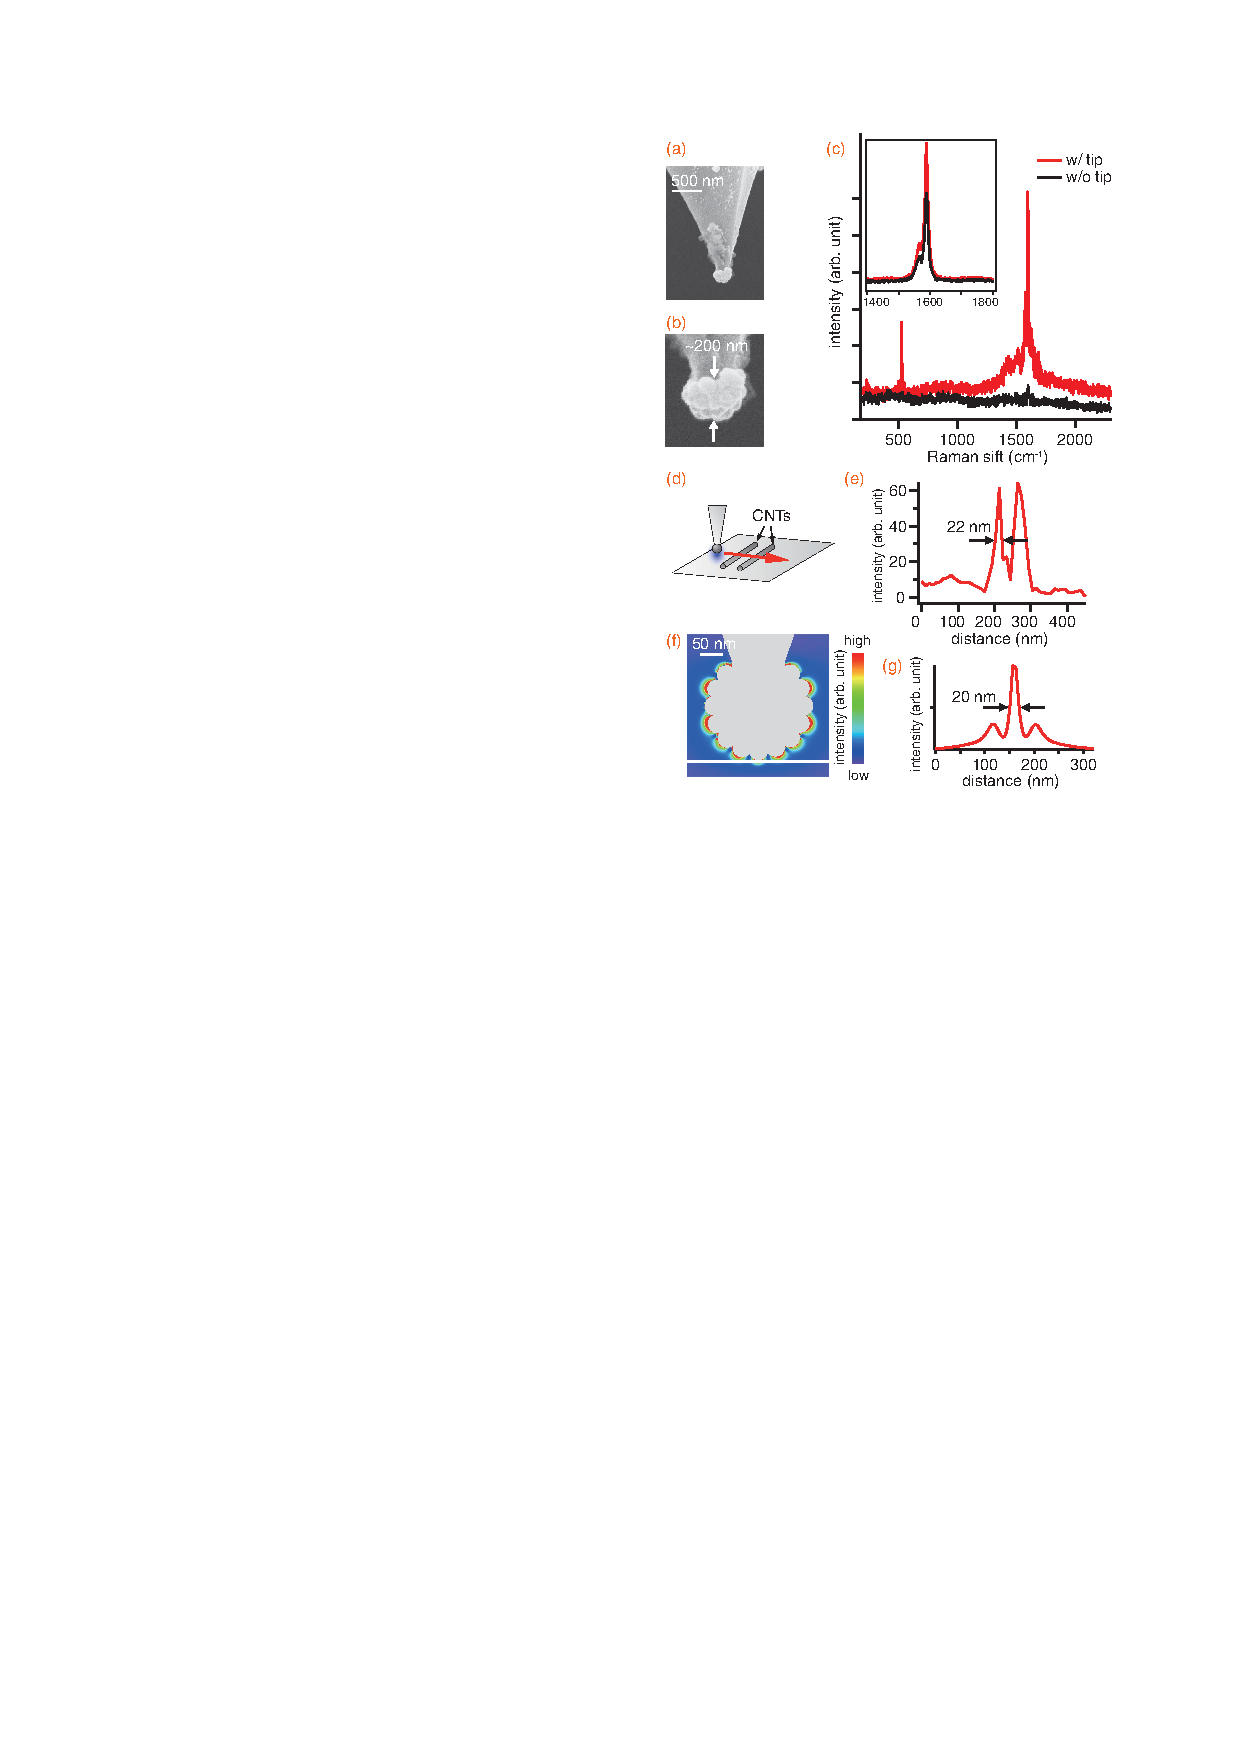
\includegraphics[width=\textwidth, clip=true, trim=0 155 0 0]{figures/literature/umakoshi2012b}
	\caption{TERS measurements and numerical simulations of AgNP-on-Si tips.}
\end{subfigure}}
{\caption[Photochemically fabricated AgNP-on-Si tips for TERS \cite{umakoshi2012}]{\textbf{Photochemically fabricated AgNP-on-Si tips for TERS \cite{umakoshi2012}.} Field enhancement is increased $\sim 20 \times$ compared with sharp Ag tips when using \SI{488}{nm} illumination with a 1.4\,NA objective in an inverted microscope.}
\label{fig:umakoshi2012}}
\end{figure}

% Non-metallic attachment
Non-metallic spherical tips on AFM probes have been created using methods such as vacuum-processing diamond-like carbon growth (NanoTools B-series) and AFM droplet pick-up \cite{}. These nanotips can then be made plasmonic through evaporation of a metallic coating.
% Metallic attachment
Other methods directly focus on structuring the apex with a solid metallic structure rather than using a post-fabrication coating.
% Concept and methods of attachment
The concept of metallic spherical nanoparticle attachment has been reported numerous times over the last decade \cite{gan2007}, beginning with the use of fibres as mounting structures \cite{kalkbrenner2001, barsegova2002, sqalli2002, kawata2003} and progressing onto the use of SPM tips \cite{umakoshi2012, hayazawa2012, park2012, okamoto2001, vakarelski2006, cheng2013}.
% Example figures
Examples of nanotips modified with metallic spherical nanostructures are shown in \figurename~\ref{fig:umakoshi2012}.

\begin{figure}
\centering
%\fcapside[\FBwidth]
{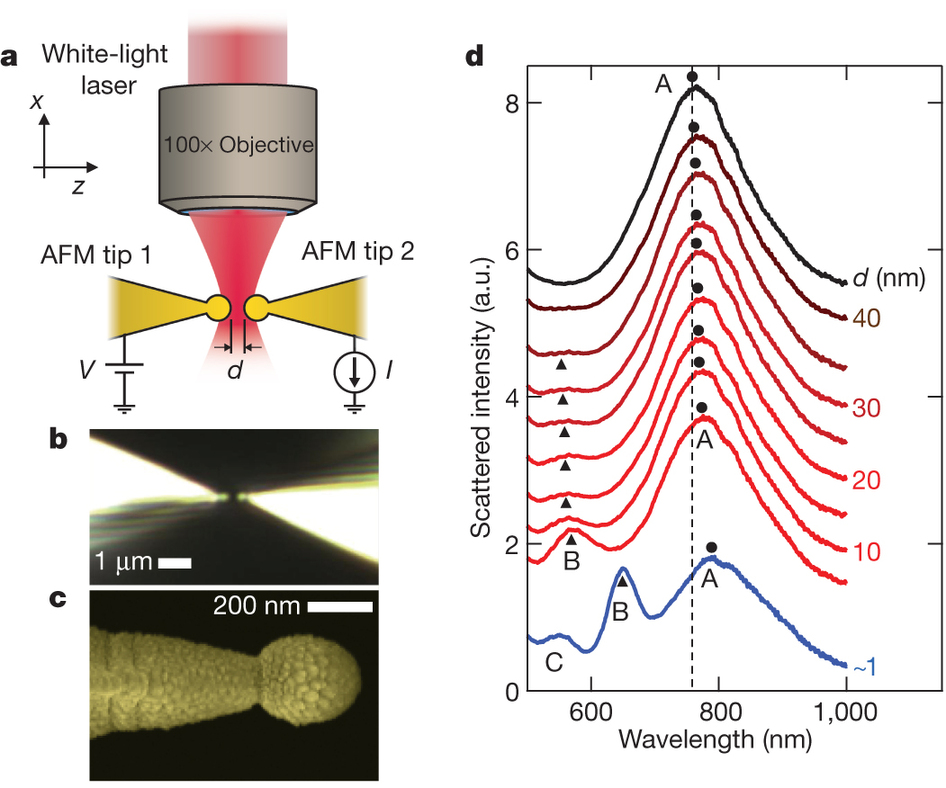
\includegraphics[width=0.65\textwidth, clip=true, trim=0 0 0 40]{figures/literature/nature11653-f1-2}}
{\caption[Experimental evidence of spherical tip plasmons and their dynamic coupling into the quantum regime of plasmonics \cite{savage2012}]{\textbf{Experimental evidence of spherical tip plasmons and their dynamic coupling into the quantum regime of plasmonics \cite{savage2012}.} Spherical tips are Au-coated NanoTools B150 AFM probes (\SI{150}{nm} radius of curvature), selected to minimise sensitivity to axial tip-tip alignment, to increase the scattered signal levels, and support higher-order plasmonic cavity modes in the visible spectrum. Resonances are far-field excited using a supercontinuum laser source in a side-illumination configuration. Separation-dependent coupling between two spherical tips confirms plasmonic behaviour.}
\label{fig:savage2012a}}
\end{figure}

% Direct measurement
Plasmon resonances in spherical tips have been observed in the far-field \cite{savage2012}, with coupling between plasmons used to confirm plasmonic behaviour.
% TERS
Furthermore a $20\times$ increase in field enhancement has been measured when using a photochemically-fabricated spherical AgNP-on-Pt tip compared with a sharp Ag tip \cite{umakoshi2012}. The increase in field enhancement also comes with an increase in {\color{red}resolution/spatial localisation}.

% Other geometries
Nanostructuring tips with other geometries has also led to an order of magnitude increase in field enhancement, attributed to LSP excitation. Electrochemical etching \cite{kharintsev2013}, FIB machining \cite{maouli2015}, selective deposition \cite{zou2009} and grafting \cite{huth2013} have successfully been used to create nanotips which are good optical antennae, especially when illuminated on resonance. Scattering resonances have been directly measured on a subset of these tips \cite{zou2009, maouli2015} while others use the field enhancement at common laser wavelengths as a measurement of antenna quality \cite{kharintsev2013}.

\cite{ichimura2009, schafer2013, pettinger2009, cherukulappurath2013, zhang2013, taguchi2009, yang2014, steidtner2007, vanschrojensteinlantman2012, angulo2011, picardi2007, uebel2013, sonntag2014, lindquist2013, mino2014, pettinger2007, ren2004, hayazawa2007, park2012, downes2006, yano2007, elkhoury2014, pettinger2009, barrios2009}
% Techniques to improve TERS such as stimulated vs. spontaneous Raman \cite{wickramasinghe2014}. Picosecond pulses \cite{klingsporn2014}
% Still to read Ichimura2009, Sch�fer2013, Pettinger2009, Cherukulappurath2013, ?Zhang2013?, Taguchi2009, Yang2014, Steidtner2007, Schrojenstein2012, ?Zhang2014?, Angulo2011, Picardi2007, Uebel2013, ?Meng?, Sonntag2014, Lindquist2013, Mino2014, Pettinger2007, Ren2004, Hayazawa2007, Park2012, Downes2006, Yano2007, El-Khoury2014, Pettinger2009, Barrios2009, Cajko2006
% Also note that thicknesses below skin depth on tips could in theory create a resonant structure since there is a dielectric on both sides.

To date there has been very little work done to reliably produce and characterise the optics of spherically nanostructured tips. Furthermore, there is still work needed to similarly measure the optical response of sharp tips, comparing them directly and quantitatively with nanostructured tips. This project focusses on developing a simple method for producing plasmonic tips with understood far-field optical responses. The comparison with sharp metallic tips can then be made and plasmonic tips applied in both fundamental studies and near-field enhancement.

\end{document}